\section{Experiments and Results}
\label{sec:results}

\subsection{Cohorts, Comparisons, and Uncertainty}
\label{sec:experimental_design}

\paragraph{PolypGen cohort and labels.}
The reviewed subset contains 5,444 frames from 37 sequences~\cite{ali2023polypgen}. Review denotes an annotation/provenance filter, not independent patient-level adjudication. A mask is positive when any pixel exceeds 127; matching bounding-box annotations must agree on presence. Unannotated frames receive negative labels only in documented negative-only sequences. Disputed center assignments and pending annotation review are excluded before fitting. This is not complete-release coverage.

Both classes occur at C2/C4/C5/C6, with 2/10/4/18 sequences, respectively. C1 has negative-only support and remains source-only; C3 is excluded after mapping review. The two encoders share the manifest, partitions, and ten fitting seeds, listed in the supplement. Architecture, pretraining, and preprocessing change together when switching encoders.

\paragraph{Histology cohort.}
The custom CAMELYON17-WILDS cohort contains 17,200 patches from 43 recorded patients, using the existing label-blind cap of 400 patches per patient and original partition~\cite{bandi2019camelyon,koh2021wilds}. Labels indicate tumor in the central $32\times32$ region of a $96\times96$ patch. H0/H3/H4 provide 26 source patients; H2 is the primary target with 9 patients and H1 the secondary target with 8. The same cohort is encoded with ResNet18, UNI, and CONCH. Both targets remain excluded from head fitting, hyperparameter selection, temperature selection, and operating-threshold selection. Standard WILDS instead uses H1 for validation and H2 for testing; our capped cohort and source-only selection define a custom representation-transfer experiment, not a full official benchmark or leaderboard result~\cite{wilds2026submission}. The foundation-encoder extension uses previously inspected hospitals and is exploratory rather than independent confirmation.


\paragraph{Prediction unit.}
Head selection uses frame/patch BA. An additional sequence readout labels presence within reviewed frames by any positive frame, scores a sequence by its maximum raw margin, and fixes its threshold by mean sequence BA at class-complete source-validation centers. C2 has two positive-bearing sequences, leaving binary sequence BA/AUROC undefined. In histology, we average within-patient patch metrics equally across patients. All target patients have positive patches; these summaries do not infer clinical patient or slide diagnoses.

\paragraph{Data ethics.}
This secondary analysis uses existing dataset releases and involves no new participant recruitment or image collection. The PolypGen authors document frame anonymization and site-specific consent and review procedures~\cite{ali2023polypgen}. The CAMELYON data collection was approved by the Commissie Mensgebonden Onderzoek regio Arnhem--Nijmegen (2016-2761), with informed consent waived~\cite{litjens2018camelyon}.

\paragraph{Experimental families and controls.}
The main experiment compares nine heads. The component analysis uses fixed $(K,\beta)\in\{1,4\}\times\{0,1\}$ and tests sensitivity to the decision threshold and source composition. The source-composition and second-encoder follow-ups are exploratory because we had inspected the original PolypGen results.

The three centroids test which unit contributes equally within a class: image, group, or center. Unbalanced multi-prototype clustering retains inverse group-size weights and fixes $\beta=0$, so its comparison with CBMP tests whether tuning center balance adds value. The linear and cosine heads learn to separate classes jointly, whereas each prototype bank fits one class at a time. Their weighted variants test group and center weighting in a discriminative objective.


CBMP's original grid has $K\in\{1,2,4,8\}$ and $\beta\in\{0,0.5,1\}$. Original candidate counts are 12/4/5/3/15/9 for CBMP, unbalanced prototypes, linear, cosine, weighted linear, and weighted cosine, with one per centroid. A second protocol uses four distinct configurations per tunable family, retaining fixed centroids. CBMP uses $\{1,4\}\times\{0,1\}$; the remaining grids are in the supplement. This changes parameter coverage as well as candidate count. Identical source fits are shared across protocols. Each PolypGen encoder supplies 880 target/head/seed evaluations. Each of the three histology encoders supplies 440, giving 3,080 evaluations across five task--encoder configurations. All use ten fitting seeds. These are repeated scores on fixed cohorts, not independent test samples or additional hospitals. The pathology extension adds representations to the existing cohort; it does not expand the patient population. The expanded grids and diagnostics remain exploratory after inspection of the original targets.

\paragraph{Metrics and uncertainty.}
Balanced accuracy (BA) is the mean of sensitivity and specificity. It gives the two classes equal weight even when a center contributes many more frames of one class. AUROC measures ranking across decision thresholds. Macro F1 summarizes thresholded predictions by class, while NLL and Brier score evaluate predicted probabilities. For the PolypGen summary, we average seed-specific metrics and then give each eligible target center equal weight. Thus C2, with 500 frames, has the same influence on mean BA as C6, with 2,187. Worst-center BA is the minimum of the four seed-averaged center scores. The supplementary materials provide per-center and per-seed metrics and selected settings.

For a paired comparison, both heads are scored on the same resampled groups in each draw. The 2,000 bootstrap attempts (seed 2027) resample whole sequences within each PolypGen target and whole patients within each histology target. We retain only class-complete draws. All predictions from a sampled group move together, preserving dependence among its recorded frames or patches. Fitted heads and the original patch selection remain fixed. The intervals quantify sensitivity to the sampled groups within the observed centers. Seed variation is reported separately because repeating a fit on the same cohort does not supply additional test patients or hospitals.

The supplementary analysis package contains the saved scores, selected settings, input hashes, and scripts needed to reconstruct the ranking diagnostics and paired contrasts.


\paragraph{Execution and assurance.}
Cached head fitting uses Python 3.12.3, NumPy 1.26.4, SciPy 1.13.1, and scikit-learn 1.5.1. UNI/CONCH extraction uses a separate Python 3.10.22/PyTorch 2.0.1+cu117 environment on a GTX 1660 Ti (6 GB), with deterministic float32 computation, batch 16 and four host threads. Source-only CPU/GPU feature checks and repeated-batch checks pass. The supplement records tolerances, environment versions, checkpoint/feature hashes and exact commands. Saved predictions and frozen source choices support reconstruction; automated checks do not replace author review.


\subsection{PolypGen: Center-Specific Transfer}
Table~\ref{tab:polypgen_results} reports ten-seed averages and fitting variation. CBMP reaches 58.05\% mean BA with ResNet18 and 59.92\% with DINOv2, versus 70.20\% for linear logistic and 68.35\% for trained cosine. Paired CBMP-minus-comparator differences are $-12.15$ points (conditional sequence-bootstrap 95\% interval $[-15.96,-8.34]$) and $-8.43$ ($[-11.27,-2.90]$). The displayed learned comparators have the highest observed target means; these conditional intervals do not adjust for selecting their names from the table.

Figure~\ref{fig:polypgen_comparison} shows the site dependence. CBMP's lowest score occurs at C5 with ResNet18 and C2 with DINOv2. DINOv2-CBMP exceeds trained cosine at C6 (77.70\% versus 73.12\%), but the center average favors cosine. Average and worst-center criteria also select different heads: ResNet18's group-weighted centroid has the strongest worst-center BA (60.34\%); DINOv2's weighted cosine leads that criterion (62.25\%). Neither is a population worst-case guarantee.

\begin{table*}[!htbp]
\centering\small
\setlength{\tabcolsep}{4pt}
\begin{tabular}{lrrrr}
\hline
Classifier & ResNet18 mean BA & ResNet18 worst BA & DINOv2 mean BA & DINOv2 worst BA \\
\hline
CBMP & $58.05\pm0.68$ & 42.17 & $59.92\pm0.48$ & 46.79 \\
Unbalanced multi-prototype & $60.99\pm0.87$ & 53.14 & $60.18\pm0.36$ & 47.85 \\
Linear logistic & $70.20\pm0.00$ & 57.17 & $61.31\pm0.00$ & 52.12 \\
Trained cosine & $63.42\pm2.46$ & 57.66 & $68.35\pm0.85$ & 61.24 \\
Weighted linear & $61.78\pm0.00$ & 47.17 & $59.24\pm0.00$ & 51.30 \\
Weighted cosine & $63.47\pm1.89$ & 45.88 & $66.75\pm2.50$ & 62.25 \\
Group-weighted centroid & $63.15\pm0.00$ & 60.34 & $64.03\pm0.00$ & 53.87 \\
Center-balanced centroid & $60.48\pm0.00$ & 47.63 & $61.21\pm0.00$ & 51.53 \\
Image-weighted centroid & $60.41\pm0.00$ & 58.17 & $62.32\pm0.00$ & 51.23 \\
\hline
\end{tabular}
\caption{PolypGen BA (percent) with the original grids. Mean BA is the mean $\pm$ fitting-seed SD of ten equal-center averages over C2/C4/C5/C6; worst BA is the minimum center-specific seed mean. The reviewed cohort contains 5,444 frames and 37 recorded sequences; patient linkage is unresolved.}
\label{tab:polypgen_results}
\end{table*}


\begin{figure*}[!t]
\centering
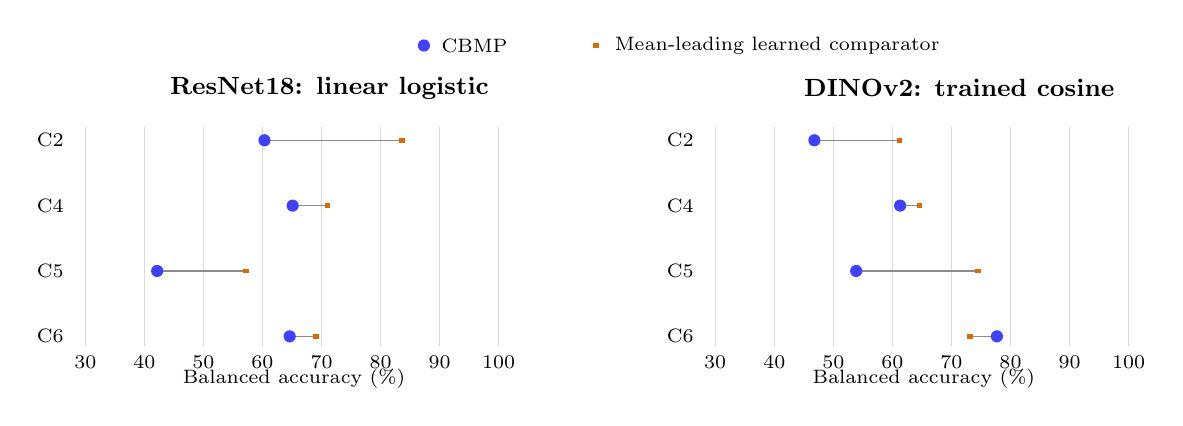
\begin{tikzpicture}[font=\scriptsize,y=.83cm]
\begin{scope}[xshift=0cm]
\node[font=\small\bfseries] at (3.1,3.8) {ResNet18: linear logistic};
\draw[black!15] (0.000000,-.15)--(0.000000,3.2);
\node[below] at (0.000000,-.15) {30};
\draw[black!15] (0.750000,-.15)--(0.750000,3.2);
\node[below] at (0.750000,-.15) {40};
\draw[black!15] (1.500000,-.15)--(1.500000,3.2);
\node[below] at (1.500000,-.15) {50};
\draw[black!15] (2.250000,-.15)--(2.250000,3.2);
\node[below] at (2.250000,-.15) {60};
\draw[black!15] (3.000000,-.15)--(3.000000,3.2);
\node[below] at (3.000000,-.15) {70};
\draw[black!15] (3.750000,-.15)--(3.750000,3.2);
\node[below] at (3.750000,-.15) {80};
\draw[black!15] (4.500000,-.15)--(4.500000,3.2);
\node[below] at (4.500000,-.15) {90};
\draw[black!15] (5.250000,-.15)--(5.250000,3.2);
\node[below] at (5.250000,-.15) {100};
\node[left] at (-.15,3) {C2};
\draw[black!45] (2.275416,3)--(4.018669,3);
\fill[blue!75] (2.275416,3) circle (2.2pt);
\fill[orange!85!black] (3.983669,2.965) rectangle (4.053669,3.035);
\node[left] at (-.15,2) {C4};
\draw[black!45] (2.632689,2)--(3.073368,2);
\fill[blue!75] (2.632689,2) circle (2.2pt);
\fill[orange!85!black] (3.038368,1.965) rectangle (3.108368,2.035);
\node[left] at (-.15,1) {C5};
\draw[black!45] (0.912446,1)--(2.037976,1);
\fill[blue!75] (0.912446,1) circle (2.2pt);
\fill[orange!85!black] (2.002976,0.965) rectangle (2.072976,1.035);
\node[left] at (-.15,0) {C6};
\draw[black!45] (2.595662,0)--(2.931159,0);
\fill[blue!75] (2.595662,0) circle (2.2pt);
\fill[orange!85!black] (2.896159,-0.035) rectangle (2.966159,0.035);
\node at (2.65,-.65) {Balanced accuracy (\%)};
\end{scope}
\begin{scope}[xshift=8cm]
\node[font=\small\bfseries] at (3.1,3.8) {DINOv2: trained cosine};
\draw[black!15] (0.000000,-.15)--(0.000000,3.2);
\node[below] at (0.000000,-.15) {30};
\draw[black!15] (0.750000,-.15)--(0.750000,3.2);
\node[below] at (0.750000,-.15) {40};
\draw[black!15] (1.500000,-.15)--(1.500000,3.2);
\node[below] at (1.500000,-.15) {50};
\draw[black!15] (2.250000,-.15)--(2.250000,3.2);
\node[below] at (2.250000,-.15) {60};
\draw[black!15] (3.000000,-.15)--(3.000000,3.2);
\node[below] at (3.000000,-.15) {70};
\draw[black!15] (3.750000,-.15)--(3.750000,3.2);
\node[below] at (3.750000,-.15) {80};
\draw[black!15] (4.500000,-.15)--(4.500000,3.2);
\node[below] at (4.500000,-.15) {90};
\draw[black!15] (5.250000,-.15)--(5.250000,3.2);
\node[below] at (5.250000,-.15) {100};
\node[left] at (-.15,3) {C2};
\draw[black!45] (1.259269,3)--(2.342641,3);
\fill[blue!75] (1.259269,3) circle (2.2pt);
\fill[orange!85!black] (2.307641,2.965) rectangle (2.377641,3.035);
\node[left] at (-.15,2) {C4};
\draw[black!45] (2.347971,2)--(2.592639,2);
\fill[blue!75] (2.347971,2) circle (2.2pt);
\fill[orange!85!black] (2.557639,1.965) rectangle (2.627639,2.035);
\node[left] at (-.15,1) {C5};
\draw[black!45] (1.790109,1)--(3.335463,1);
\fill[blue!75] (1.790109,1) circle (2.2pt);
\fill[orange!85!black] (3.300463,0.965) rectangle (3.370463,1.035);
\node[left] at (-.15,0) {C6};
\draw[black!45] (3.577295,0)--(3.234098,0);
\fill[blue!75] (3.577295,0) circle (2.2pt);
\fill[orange!85!black] (3.199098,-0.035) rectangle (3.269098,0.035);
\node at (2.65,-.65) {Balanced accuracy (\%)};
\end{scope}
\fill[blue!75] (4.3,4.45) circle (2.2pt);
\node[right] at (4.4,4.45) {CBMP};
\fill[orange!85!black] (6.45,4.415) rectangle (6.52,4.485);
\node[right] at (6.6,4.45) {Mean-leading learned comparator};
\end{tikzpicture}
\caption{Center-specific PolypGen BA averaged across ten fitting seeds using the original grids. Connectors pair point estimates, not confidence intervals. The displayed learned comparator has the highest observed target mean within its encoder.}
\label{fig:polypgen_comparison}
\end{figure*}




\paragraph{Component diagnostics.}
Mean BA at $(K,\beta)=(1,0),(1,1),(4,0),(4,1)$ is 63.15\%, 60.48\%, 59.78\%, 59.42\% for ResNet18 and 64.03\%, 61.21\%, 64.48\%, 60.12\% for DINOv2. The balancing effect at $K=4$ minus its effect at $K=1$ is $2.31$ points for ResNet18 (paired 95\% interval $[-0.09,7.23]$) and $-1.54$ for DINOv2 ($[-6.57,4.07]$). Both intervals include zero. These ten-seed results do not resolve a uniform mean-BA interaction between multiplicity and balancing.

\paragraph{Tuning sensitivity.}
With four configurations per tunable family, CBMP reaches 60.56\% mean BA with ResNet18 and 60.25\% with DINOv2; linear (70.20\%) and cosine (68.22\%) remain the leading learned heads. The reduced grids change parameter coverage as well as count. Full paired sensitivity results are in the supplement.

\paragraph{Sequence readout.}
For the same frame-selected heads, the source-thresholded sequence rule gives mean BA over C4/C5/C6 of 39.25\% versus 70.14\% for ResNet18-CBMP versus linear, and 67.78\% versus 60.07\% for DINOv2-CBMP versus cosine. The latter point ordering differs from frame BA, but its paired difference of $+7.71$ points has interval $[-4.81,19.84]$. Aggregation, labels, and operating points change together. Sparse group support and sequence-length effects limit interpretation; C2 remains undefined at this binary endpoint.


\subsection{CAMELYON17-WILDS: Frozen Pathology Encoders}
\label{sec:pathology_foundation}

We compare ResNet18, UNI, and CONCH on the same custom cohort, with identical target identities, source folds, head families, and fitting seeds. Table~\ref{tab:foundation_heads} focuses on the four-candidate source-only protocol. Historical-grid results and the full nine-head comparisons are reported separately. All heads are frozen and hashed before either target hospital is scored.

\begin{table}[t]
\centering\small
\setlength{\tabcolsep}{3pt}
\begin{tabular}{llrrr}
\hline
Target & Encoder & CBMP & Linear & Cosine \\
\hline
H2 & ResNet18 & 85.54 & 88.88 & 86.73 \\
   & UNI      & 95.80 & 97.72 & 97.96 \\
   & CONCH    & 92.63 & 96.50 & 96.88 \\
\hline
H1 & ResNet18 & 77.14 & 80.30 & 78.90 \\
   & UNI      & 95.02 & 97.47 & 97.48 \\
   & CONCH    & 93.79 & 92.88 & 93.95 \\
\hline
\end{tabular}
\caption{Patch balanced accuracy (\%), averaged over ten fitting seeds on identical sampled patients under the four-candidate protocol. H2 is primary and H1 secondary. Linear denotes logistic regression; cosine denotes the trained cosine head. These three heads are a focused view; all nine heads, fitting-seed SDs, AUROC, and the historical-grid controls are reported separately. This is the custom CAMELYON17-WILDS cohort.}
\label{tab:foundation_heads}
\end{table}


\paragraph{Representation changes and classifier differences.}
At primary H2, trained cosine reaches 97.96\% BA with UNI and 96.88\% with CONCH, versus 86.73\% with ResNet18. CBMP reaches 95.80\%, 92.63\%, and 85.54\%, respectively. Both pathology encoders increase the displayed point estimates, while learned heads retain higher primary-target BA than source-selected CBMP. Encoder-associated gains therefore do not establish an advantage for prototype balancing or multiplicity. AUROC and all-head comparisons are provided in the supplement.

\paragraph{Paired target uncertainty.}
The H2 CBMP-minus-linear BA difference is $-1.92$ points for UNI (conditional patient-bootstrap 95\% interval $[-5.76,-0.07]$) and $-3.87$ for CONCH ($[-10.48,-0.52]$). At secondary H1, CONCH-CBMP reaches 93.79\% BA versus linear's 92.88\%; its $+0.91$-point interval $[-0.50,2.27]$ includes zero. These exploratory intervals use 2,000 paired patient-resampling attempts with fitted heads fixed, without adjustment for multiple comparisons. They do not quantify a population of hospitals.

\paragraph{Which prototype rule was selected?}
Under the four-candidate protocol, source validation selects $(K,\beta)=(1,1)$ for CONCH in all ten fitting seeds. Its selected CBMP therefore reduces to the center-balanced single-centroid case; the reported score is not evidence for a benefit from multiple prototypes. UNI instead selects $K=4$ in all ten seeds, with $\beta=0$ in seven and $\beta=1$ in three. The effective prototype rule depends on the representation and source-validation evidence. These selected configurations motivate reporting both the chosen rule and fixed $(K,\beta)$ controls; they do not establish why the selected rule transfers or fails at a particular hospital.



\subsection{Where Does Ranking Break Down?}
\label{sec:group_ranking}
Unless stated otherwise, the ranking and patient-weighting diagnostics below use the original candidate grids. The foundation-encoder comparison in Section~\ref{sec:pathology_foundation} uses the four-candidate sensitivity protocol. The two sets of point estimates should therefore not be interchanged.
Group-specific ranking has a precedent in covariate-adjusted ROC analysis~\cite{janes2009adjusting}. For each held-out center and fitting seed, we compare the positive-class scores of every positive--negative image pair. We record a win when the positive image scores higher and half a win for a tie. The same-group component asks whether a head separates the classes within sequences or patients containing both labels. The across-group component asks whether scores remain comparable between two distinct groups. If $\rho$ is the share of pairs drawn from the same group, then
\begin{equation}
    A_{\mathrm{pooled}}=\rho A_{\mathrm{same}}+(1-\rho)A_{\mathrm{across}}.
    \label{eq:ranking_decomposition}
\end{equation}
A component is undefined when it has no eligible pairs, and such a component contributes zero weight to the pooled score.

Ordinary AUROC implicitly gives a positive group with $n_g^+$ images and a negative group with $n_h^-$ images weight proportional to $n_g^+n_h^-$. Equal group-pair AUROC averages observed ordered group pairs uniformly. Class-support inspection identifies removals that make the endpoint undefined. All diagnostics use fixed scores and decisions after fitting. Factorial contrasts use 2,000 sequence-resampling attempts shared across settings, seeds, and encoders. We retain draws with the relevant component defined and report their counts alongside the intervals.

\begin{table}[!htbp]
\centering\small
\setlength{\tabcolsep}{4pt}
\begin{tabular}{llrrrr}
\hline
Site/encoder & Head & Pooled & Same & Across & Equal \\
\hline
C5 / ResNet18 & CBMP & 43.87 & 93.22 & 40.43 & 52.59 \\
 & Linear & 65.10 & 91.56 & 63.26 & 71.47 \\
C5 / DINOv2 & CBMP & 57.90 & 94.86 & 55.33 & 64.29 \\
 & Cosine & 81.95 & 94.13 & 81.10 & 84.52 \\
H2 / ResNet18 & CBMP & 92.54 & 91.85 & 92.59 & 86.00 \\
 & Linear & 95.14 & 94.06 & 95.21 & 86.26 \\
\hline
\end{tabular}
\caption{Ranking diagnostics with the original grids (percent), averaged over ten fitting seeds. Same/Across distinguish recorded group identity; Equal assigns uniform weight to observed group pairs. C5 has one positive-bearing sequence; H2 is the primary histology target.}
\label{tab:group_ranking}
\end{table}



\paragraph{The selected rule.}
At C5, all ten DINOv2 fits select $(K,\beta)=(1,0)$, a group-weighted centroid. An independent calculation through explicit source-group means verifies this analytic limit; its failure there is not unstable multi-prototype optimization. All 199 target positives belong to one sequence, with 51 negatives there and 731 in the other three. Same-sequence pairs have weight 6.52\% in Eq.~\ref{eq:ranking_decomposition}, combining 94.86\% Same and 55.33\% Across AUROC into 57.90\% pooled AUROC. All ten ResNet18 fits instead select $(2,1)$ at C5, so the observed rules have different mechanisms.

The negative populations also differ: within the mixed sequence they are frames of a polyp-bearing recording, while the others belong to negative-only released sequences~\cite{ali2023polypgen}. Case mix and between-sequence score shifts are both compatible with the contrast. Removing C5's sole positive-bearing sequence or C2's sole negative-bearing sequence makes frame BA and AUROC undefined. The diagnostic locates a difference without establishing its clinical cause.


\paragraph{Fixed choices and source selection.}
Holding $K=4$ fixed at C5, DINOv2 balancing changes Same AUROC from 95.17\% to 95.43\% and Across from 76.91\% to 51.30\%. The Across difference is $-25.61$ points (conditional paired 95\% interval $[-45.59,-13.28]$, 1370 valid draws). The ResNet18 difference is $-7.55$ ($[-21.16,-2.48]$). Table~\ref{tab:factorial_ranking} gives all targets; effects vary with site and encoder.

\begin{table}[!htbp]
\centering\small
\setlength{\tabcolsep}{4pt}
\begin{tabular}{llrr}
\hline
Encoder & Target & $\Delta$Same & $\Delta$Across \\
\hline
ResNet18 & C2 & -0.92 & -5.20 \\
ResNet18 & C4 & +7.57 & -0.37 \\
ResNet18 & C5 & +10.84 & -7.55 \\
ResNet18 & C6 & +4.03 & -1.34 \\
DINOv2 & C2 & +7.70 & -7.92 \\
DINOv2 & C4 & +2.11 & +1.19 \\
DINOv2 & C5 & +0.26 & -25.61 \\
DINOv2 & C6 & +1.13 & +0.80 \\
\hline
\end{tabular}
\caption{AUROC change (points) from $\beta=0$ to $\beta=1$ at fixed $K=4$, averaged over ten fitting seeds. Paired conditional intervals and valid-draw counts are supplied in the report and supplement.}
\label{tab:factorial_ranking}
\end{table}



Source selection also matters. At C5, DINOv2's $(1,0)$ setting has 68.00\% mean inner source BA, versus 58.00\% for $(4,0)$. Their target BA is 53.87\% versus 76.24\%. This reversal diagnoses a mismatch between source validation and the observed target. The source-selected head stays fixed throughout the analysis.


\paragraph{Histology and patient weighting.}
With ResNet18 and the original grids, equal patient-pair weighting at H2 changes the CBMP-minus-linear AUROC gap from $-2.59$ points to $-0.26$ with scores unchanged. Patient-macro patch BA is 79.04\% versus 80.27\%, with paired difference $-1.23$ ($[-3.98,2.71]$). At H1 the point ordering reverses: 71.35\% versus 70.15\%, or $+1.20$ ($[-3.35,6.75]$). Both macro-BA intervals include zero. These summaries expose dependence on patient weighting; they do not infer clinical patient diagnosis. Full results for both hospitals accompany the report.


\subsection{Interpretation and Limits}
The algorithmic contrasts locate ranking changes when prototype construction changes, without identifying an acquisition or clinical cause. A uniform group-score shift preserves Same AUROC. Case mix and between-group comparability therefore deserve separate examination rather than attribution to a single nuisance factor.

At C5, resampling reuses one positive-bearing sequence; at C2, Across has one observed group pair. Zero-width conditional intervals can reflect that restricted support. Only 1,026 of 2,000 PolypGen draws retain both frame classes at every target. PolypGen patient linkage and excluded mappings remain unresolved. The earlier three-seed sequence-removal stress analysis is observational and inconclusive. All target-driven diagnostics remain exploratory.

The pathology foundation-encoder comparison addresses representation coverage on the existing cohort, but adds no patients or hospitals. Its conclusions remain conditional on 9 primary and 8 secondary target patients, with no hospital-population inference. Absence of overlap between provider pretraining data and this cohort has not been independently established. The comparison is exploratory because these hospitals had already been inspected. More fitting seeds quantify variability on these same observations; they do not provide independent confirmation. Full official-split evaluation, a modern DG training comparison, resolved PolypGen patient linkage, and an untouched patient-linked cohort remain separate requirements.


